\documentclass[a4paper]{article}
\usepackage{ctex}
\usepackage{multicol}
\usepackage{fancyhdr}
\usepackage{color}
\usepackage{CJK}
\usepackage{amsmath}
\usepackage{graphicx}
\usepackage{algorithm}%写算法时需要调用的包
\usepackage{algorithmic}%写算法时需要调用的包
\usepackage{setspace}%修改行间距需要调用的包
\usepackage{graphicx}
\definecolor{gray}{RGB}{192,192,192}%灰色设置
\title{\heiti \Large 我的五子棋AI果然有问题}%题目
\author{\songti \small 韩梓辰\ 夏星晨\ 周贤玮\ 赵云龙\ 张坤龙}%作者信息
\pagestyle{fancy}
\lhead{\textcolor{gray} {Computer Science 计算机科学}}
\rhead{\textcolor{gray} {\thepage}}
\renewcommand{\headrulewidth}{0.4pt}
\begin{document}
\maketitle %标题
\thispagestyle{fancy} %页眉
\lhead{\textcolor{gray} {计算机科学}}
\rhead{\textcolor{gray} {DOI:xxxxxx}}
\renewcommand{\headrulewidth}{0.4pt}
\begin{abstract}
    近年来,AlphaGo在棋坛上打遍天下无敌手,甚至进军电子竞技行业,人工智能在发展到今天,人类在竞技体育领域可能越来越不是他们的对手。但是,显然光对胜利的渴求并不新颖,因为人工智能现在越来越多的在各个领域聪明,从以前的人工智障变成了人工智能,在去年,日本一个公司开发了一款人工智能,号称史上最弱人工智能,这个人工智能在几百万次的游戏对战中只获取了1000次的胜利,无论人类如何放水,这个人工智能反倒越来越弱。于是放弃原有的老套人工智能思路,改为设计“人工智障”成为了一个全新的设计思路。\par
该五子棋“人工智障”将基于Python编程语言,通过数学建模,博弈树,神经网络等算法实现。使用pytorch工具,CUDA加速实现矩阵运算的优化,更加优秀的卷积神经网络设计等方法对其进行进一步的优化。最后,在通过大量的人机对战、机机对战、预设对战的数据的学习下,该人工智障已具备一定的计算机科学技术上的智能水平,具有了一定的研究与使用意义。
    \par\textbf{关键词:\ }人工智能,五子棋,神经网络,人工智障,TensorFlow
\end{abstract}
\setlength{\baselineskip}{20pt}
\tableofcontents  %表示目录部分开始
\newpage
    \begin{multicols}{2}
    \section{引言}
    在计算机科学高速发展的当代,人工智能的上限已经变成了一个未知数。人工智能之父图灵在1950年曾说过:下棋是很抽象的活动,是机器可以和人竞争的纯智能领域之一。\cite{ref1}自此之后,越来越多的学者开始研发超越人类的AI,攻克那些曾让人类引以为傲的脑力项目。在1997年时, IBM研发的Deeper Blue战胜了当年国际象棋世界冠军卡斯帕罗夫, 成为人工智能挑战人类智慧发展的里程碑。\cite{b1}而2016 年 3 月,谷歌研发的人工智能–阿尔法狗与围棋世界冠军、职业九段棋手李世石进行围棋人机大战,以4 比 1 的总比分获胜,震惊了棋坛;2016 年末 2017 年初,该程序在中国棋类网站上以“大师” (Master)为注册账号与中日韩数十位围棋高手进行快棋对决,连续 60 局无一败绩,当人们知晓的时候,无不对人工智能的力量感到佩服;2017 年 5 月,在中国乌镇围棋峰会上,它与排名世界第一的世界围棋冠军柯洁对战,以 3比 0 的总比分获胜,取得了围棋界的王冠。围棋界公认阿尔法围棋的棋力已经超过人类职业围棋顶尖水平。\cite{b3}人工智能在棋类方面令人诧异的表现将它推上了一个新的高度。时至今日,棋类AI的算法技术趋向成熟,大量的优化算法,学习模型的构建被提出、完善,包括决策树,算杀,A*搜索等等。这让人工智能在棋类方面几乎变得无懈可击。\cite{b2} \par
就在去年,日本“AVILEN”AI技术公司的首席技术官吉田拓真却反其道而行,研发出了一款“最弱AI”。针对这个模型,他构建了五层神经网络,盘面信息为输入层,输出的是棋盘有利度,通过模仿AlphaGO的构建,以及使用的算法,他成功做出了这个号称“史上最弱”的人工智能。他在推特上发表了这款支持人机对战的黑白棋小程序,最终,这个黑白棋AI在上千名网友的挑战下只输了寥寥数次。这打破了原本“创造胜过人类的人工智能”的固有思维模式。然而,出于时间原因,吉田拓真仅制作了黑白棋的AI程序\cite{ref2},而目前,在其他棋类游戏方面的“人工智障”还是一片空白。\par
基于这个创意,本组决定转换方向,即通过反向思路实现,将人工智能彻底做成另一个新的方向,即“人工智障”。我们计划设计一款可以不断的被人类战胜的机器,无论人类如何放水都可以输掉整个比赛。,本组决定以博弈树,极大极小值搜索,算杀等较为普遍的算法为基础,通过更加优秀的数学建模,神经学习网络,底层优化来实现本组预期制作的五子棋“人工智障”。并将以人与AI,AI与AI之间的棋局胜负为指标,来验证本组五子棋AI的优越性。
    \section{相关工作}
    \subsection{python学习}
    由于大家对python编程语言并不是很熟悉,所以在项目初期,我们五个人都进行了python的学习\cite{ref3},通过python的短暂学习,大家均掌握了大部分的python语法,包括pip的安装库,for的高级用法。通过在网站上的学习过程,我们逐渐的学习并熟练了python的过程,我们利用pygame对本次五子棋的图形界面进行了实现。
    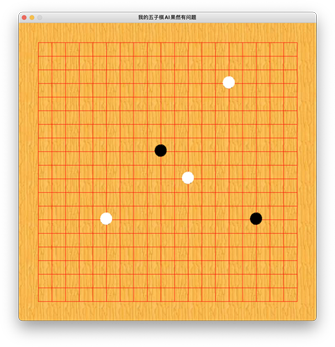
\includegraphics[width=6cm,height=6cm]{gamepic.png}
    此版本游戏实现较为简陋,后期我们对棋子的图片进行了重制,并兼顾了ai的算力的影响等问题,实现了第二版的图形界面,第二版的效果如下:
    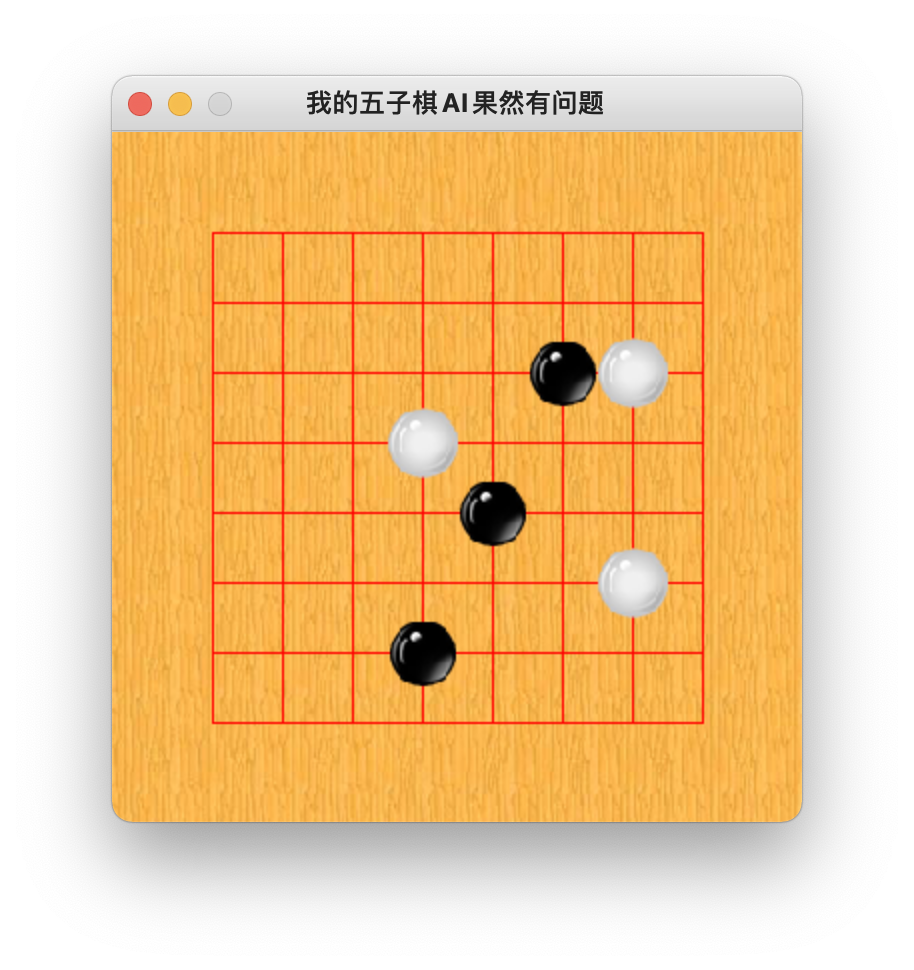
\includegraphics[width=6cm,height=6cm]{game.png}
    \subsection{对照算法}
在训练神经网络之前,我们需要一个标准算法对我们的模型进行训练,这里我们采用的是蒙特卡洛树搜索。
\subsubsection{算法概述}
蒙特卡洛树搜索其实并非什么新型算法,早在上个世纪四十年代,为了满足原子能事业的发展,这个算法就已经被投入使用\cite{k1}。而直到2016 年 3 月,谷歌研发的人工智能–阿尔法狗与围棋世界冠军、职业九段棋手李世石进行围棋人机大战,最终以4 比 1 的总比分获胜,它才引起了人们的注意,网上也开始出现各种博客、论文等详细解析这个算法。时至今日,蒙特卡洛树搜索已经在棋类游戏AI中被广泛使用。\par
蒙特卡洛树搜索实际上是一种随机模拟与树的搜索的结合\cite{k2},它最大的优点它能权衡探索与利用,是一个在搜索空间巨大仍然比较有效的的搜索算法。对于传统的树搜索算法来说,
如果搜索层数较浅,我们就可以照常穷举出所有的情况,得到每一个树节点输赢的概率,然后通过最大最小值搜索得到一个纳什均衡点。然而对于搜索层数比较深的情况(如一
个$10*10$棋盘的五子棋),若要遍历每一个棋局的每一种情况,所有可能的状态将近$3^{100}$个\footnote{对于棋盘上每个点有三种情况:白子,黑子,无子,一共有100个棋格,故大致估算为$3^{100}$种情况(约为$5.15*10^{47}$种情况)},这是现有的计算机无法承受的。这个时候,我们就需要蒙特卡洛树搜索,来帮助我们进行抉择,随机抛弃
一些节点,再进行搜索。这样虽然不能得到所有点的权重,但是可以在有限的时间内换取更多胜率更高的点,从而抛弃大量冗余的节点,节省下大量的时间。
\subsubsection{算法实现}
我们设一个节点i的价值为vi(我们可以使用各种公式来决定函数v,比如最简单的 胜利局数/总局数,或者使用Upper Confidence Bounds(UCB)公式\footnote{Upper Confidence Bounds(UCB)公式:$V_{i}+C*\sqrt{\frac{lnN}{n_{i}}}$)其中 $V_{i}$是节点的估计价值,$n_{i}$是节点被访问的次数,而N则是其父节点已经被访问的总次数。C是一个可调整参数,类似于Perception中的learning rate,它决定了在我们进行蒙特卡洛树搜索时,遍历的次数对该节点估值的影响大小。\par}。大部分的蒙特卡洛树搜索包含一下四个阶段\cite{k3}:\par
1.	选择(Selection)
在这一步,我们会从树的根节点开始,每次都选择一个“最值得我们搜索的点”,即vi最大的子节点,直到我们遇见一个存在未被扩展的子节点的节点。然后我们就对该节点进行扩展。如下图,假设我们遍历到了5号点。\par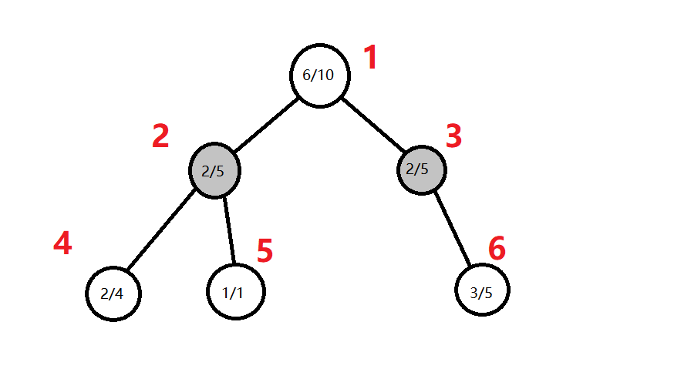
\includegraphics[width=6cm,height=6cm]{k1.png}
2.	扩展(Expansion)
我们新建立一个子节点7作为5号节点的扩展(如图二)。值得注意的是,如果我们当前遍历到的点是白点(这代表此时轮到白方执子),子节点的建立必须是一个黑点(因为此时已经轮到黑方执子)。接着进入第三步模拟。此外,我们的拓展需要有一定的随机性,而非仅仅是按照字典序排序,来保证蒙特卡洛树搜索能充分扩展到“最有搜索价值”的节点\footnote{我们考虑这样一种情况:如果在某一个节点i的胜率很高,可能是50/100,而另一个节点j的胜率也有40/80。那么此时,我们会选择i节点进行扩展。当i节点胜利之后,我们会再次搜索到i节点。如果这次的搜索失败了,那么它的胜率依旧是1/2。在我们不采用随机数的情况下,根据字典序,我们还是会选择节点i来扩展。这就导致了一个循环,i节点在不断被扩展,而j节点一直不会被访问到——即使j的实际胜率可能远远高于i节点。}。\par
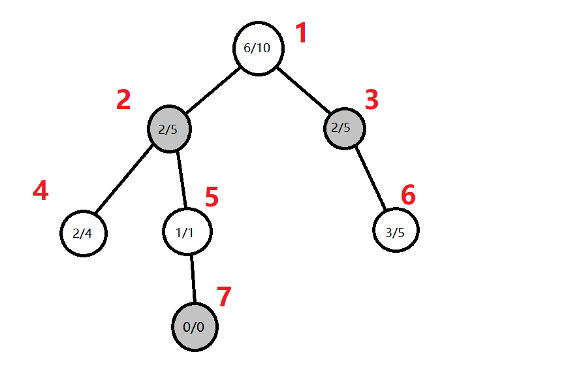
\includegraphics[width=6cm,height=6cm]{k2.png}
3.	模拟(Simulation)
在这个步骤中,我们通过某种特定的下子方法(如仅仅是优秀的随机,甚至于连杀,连防\footnote{连杀、连防:这二者都是五子棋中一种最基础的下法,它不需要大量的思考与计算,但是却非常地接近最优解。所以对于新手而言,连杀与连防是想要下好五子棋必须掌握的策略。具体来说,连杀是指对于进攻方的每一次落子,都能形成活三/眠四/三三/四三/四四,从而逼迫对手进行连防。连防也是一个相似的概念,它是指对于防守方的每一次落子,都能将对手的活二/活三/眠四转变为眠二/眠三/死四。当防守方的防守做得足够优秀,进攻方就无法产生足够大的压力,此时就可以选择一转攻势,通过连杀尝试将对手杀棋。}),来快速走子,获得最后的胜负情况,更新到7节点上(如图3)。\par
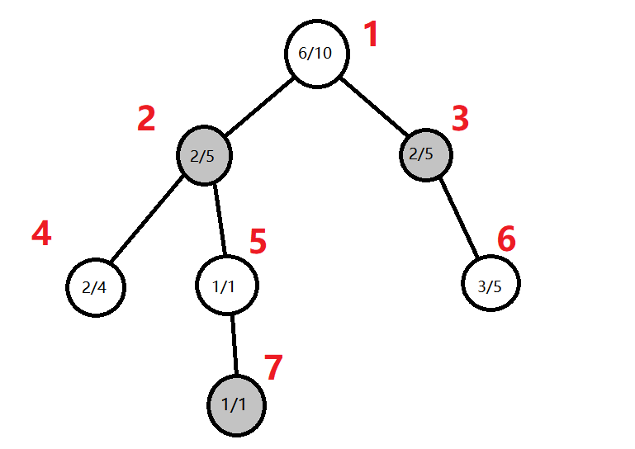
\includegraphics[width=6cm,height=6cm]{k3.png}
4.	反演(Backpropagation)
从7号点出发,将获得的结果回溯到父节点上,更新每一个节点的胜负情况,如图4。需要注意的是,白点代表白子,灰点代表黑子,所以更新的时候若黑点胜利则父白点应记为失败,反之亦然。\par
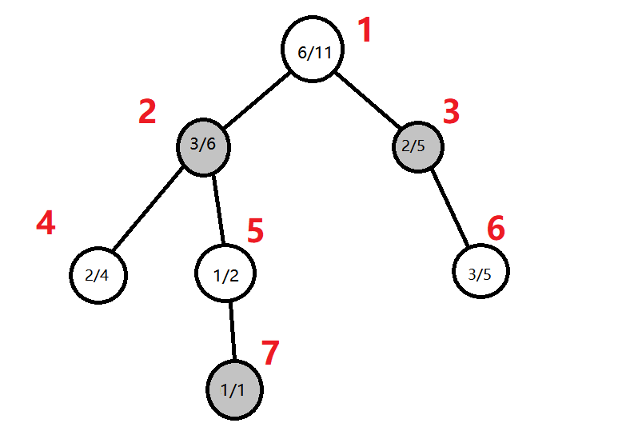
\includegraphics[width=6cm,height=6cm]{k4.png}
5.	重复步骤1。蒙特卡洛树搜索可以在任何时候停止,它的准确度随着搜索时间的增加而收敛。一般来说,我们也会通过设定搜索深度的限制来防止节点任意地拓展,减缓运行的速度。\par
\subsubsection{算法优点}
蒙特卡洛树搜索具有很多的优点\cite{k4}:\par
1.	泛用性。蒙特卡洛树搜索并不要求有太多的专业知识,只要了解了基本的规则,就能很好地完成它的任务。这使得蒙特卡洛树搜索只要稍加更改就能用于另一个模型。\par
2.	非对称的扩展。\cite{k5}MCTS 执行一种非对称的树的适应搜索空间拓扑结构的增长。这个算法会更频繁地访问更加有趣的节点,并聚焦其搜索时间在更加相关的树的部分。非对称的增长这使得 MCTS 更加适合那些有着更大的分支因子的博弈游戏,比如说 19X19 的围棋。这么大的组合空间会给标准的基于深度或者宽度的搜索方法带来问题,所以 MCTS 的适应性说明它(最终)可以找到那些更加优化的行动,并将搜索的工作聚焦在这些部分。
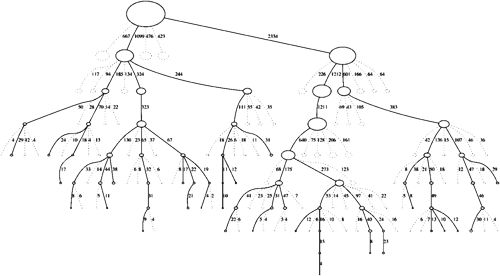
\includegraphics[width=6cm,height=6cm]{k4.jpg}
\par
3.	可被终止。算法可以在任何时候被终止,此时会返回目前所得的最优解。\cite{k6}\par



    \section{程序代码}

    \section{验证}

    \section{结束语}

    \newpage
    \addcontentsline{toc}{section}{参考文献}
    \begin{thebibliography}{30}%参考文献
    \bibitem{ref1}{李金洪\ 深度学习之TensorFlow\ [M]\ .北京.机械工业出版社, 2018-3}
    \bibitem{b1}{ 陈东焰,陆畅.从AlphaGo看机器学习[J].科技创新导报,2020,17(13):146-148. }
    \bibitem{b3}{百度百科 AlphaGo }
    \bibitem{b2}{计算机围棋AlphaGo算法对人类围棋算法的影响[J]. 程思雨,林锋.  中国科技信息. 2019(02)}
    \bibitem{ref2}{naka. J., The weakest Othello, Takujin Yoshida.Thoroughly dig into the inside of the development!(2019-7-25) [2020-09-01]https://ai-trend.jp/business-article/interview/othello-cto-interview}
    \bibitem{ref3}{python基础教程 https://www.runoob.com/python/python-tutorial.html}
    \bibitem{ref4}{董慧颖;王杨.多种搜索算法的五子棋博弈算法研究[J].沈阳理工大学学报,2017,2}
    \bibitem{k1}{沈大旺.基于人工智能的五子棋搜索算法[J].产业与科技论坛,2020,19(01):73-74.
http://nooverfit.com/wp/%E8%92%99%E7%89%B9%E5%8D%A1%E6%B4%9B%E6%A0%91%E6%90%9C%E7%B4%A2-mcts-%E5%85%A5%E9%97%A8/
}
    \bibitem{k2}{知乎;匿名用户 蒙特卡洛树是什么算法?2017-05-09 https://www.zhihu.com/question/39916945}
    \bibitem{k3}{刘建平Pinard的博客 强化学习(十八) 基于模拟的搜索与蒙特卡罗树搜索(MCTS) 2019-03-04 https://www.cnblogs.com/pinard/p/10470571.html}
    \bibitem{k4}{yif25博客 蒙特卡罗树搜索(MCTS)2018-01-17 16:07 https://www.cnblogs.com/yifdu25/p/8303462.html}
    \bibitem{k5}{知乎; Xiaohu Zhu 蒙特卡洛树搜索简介 https://zhuanlan.zhihu.com/p/30316076}
    \bibitem{k6}{基于蒙特卡洛树搜索的计算机围棋博弈研究[D]. 于永波.大连海事大学 2015}

    \end{thebibliography}
    \newpage
\end{multicols}
\end{document}
